%
% einleitung.tex -- Beispiel-File für die Einleitung
%
% (c) 2020 Severin Weiss
%
Die Laplacetransformation einer auf $[0, \infty)$ definierten und in jedem endlichen Intrevall $[0, a)$ absolut integrierbaren Funktion, ist die Funktion
\begin{equation}
F(s) = \int_0^\infty e^{-st}f(t)\,dt,~~Re(s)>\gamma_{0}.
\label{laplace:definition}
\end{equation}
Das Argument $s$ kann eine komplexe Zahl sein, im Folgenden wird vorausgesetzt, dass das Integral für $Re(s)>\gamma_{0}$ konvergieren muss.
Das inverse Laplaceproblem ist, die Funktionen $f(t)$ im Zeitbereich aus jener bekannten Funktionen $F(s)$ im Frequenzbereich zu rekonstruieren.

Mit der Riemanninversionsformel ergibt sich $f(t)$ aus $F(s)$
\begin{equation}
f(t) = \frac{1}{2\pi i} \oint_{B} e^{st}F(s)\,ds,~~t>0
\label{laplace:riemanninversionsformel}
\end{equation}

wobei $B$ die Bromwichkontur von $\gamma-i\infty$ bis $\gamma+i\infty$, mit $\gamma>\gamma_{0}$, parallel zur imaginären Achse ist. Die Bromwichkontur ist eine geschlossen Kurve. Die Kurve ist in Abbildung \ref{laplace:bromwichkontur} ersichtlich. Sie besteht aus zwei Teilen. Zum einen der Teilkreis mit Radius $R$ vom Mittelpunkt und zum anderen der vertikalen Linie $\gamma$, welche sich zur rechten aller Singularitäten von $F(s)$ befindet.  Bei Vergrösserung des Radius $R$ wird die Bromwichkontur alle Singularitäten umschliessen. Unter diesen Bedingung konvergiert das Integral gegen Null, wenn der Radius $R$ gegen unendlich strebt.
Damit man das Integral mit der Bromwichkontur numerisch berechnen kann, braucht man $F(s)$, sodass für alle $s\rightarrow$ $\infty$ mit $Re(s)> \gamma_{0}$ genügend schnell gegen 0 gehen, weil der Umfang des Kreises anwächst.


\begin{figure}
\centering
%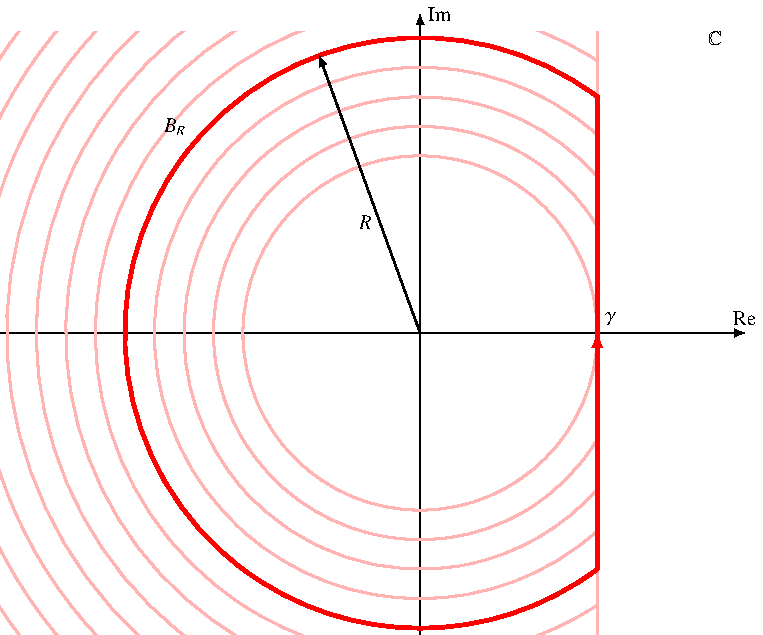
\includegraphics[width=6.9cm]{papers/laplace/images/bromwich.pdf}
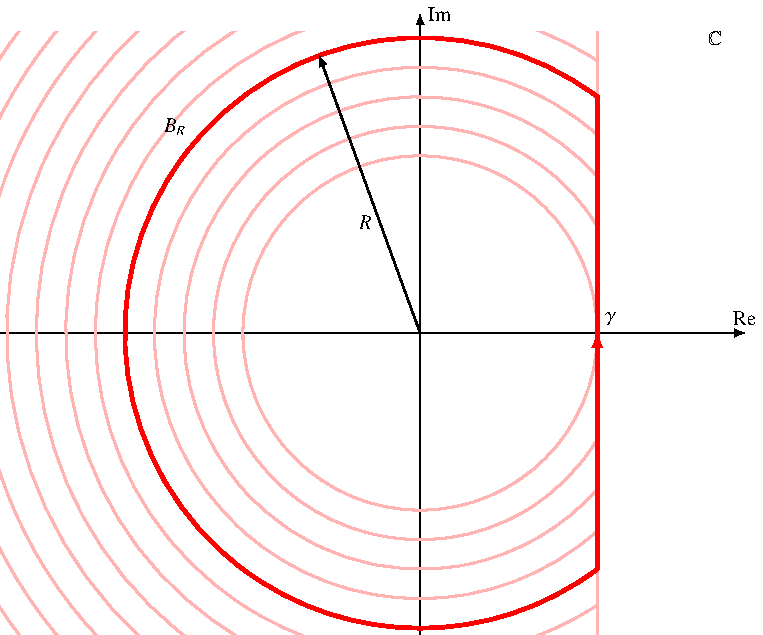
\includegraphics{papers/laplace/images/bromwich.pdf}
\caption{Die Bromwichkontur in der komplexen Ebene. Dargestellt ist die wachsende Figur abhängig vom Radius $R$.
\label{laplace:bromwichkontur}
}
\end{figure}

Im Allgemeinen möchte man die Kontur zur linken Seite bewegen, sodass der Betrag des Faktors $e^{st}$ im Integrand kleiner wird.
Die Kontur sollte jedoch nicht zu nahe an Singularitäten von $F(s)$ angenähert werden, dies würde Spitzen des Integranden zur Folge haben.

